\subsection{Begriffserkl"arungen}

\begin{figure*}[b]
	\centering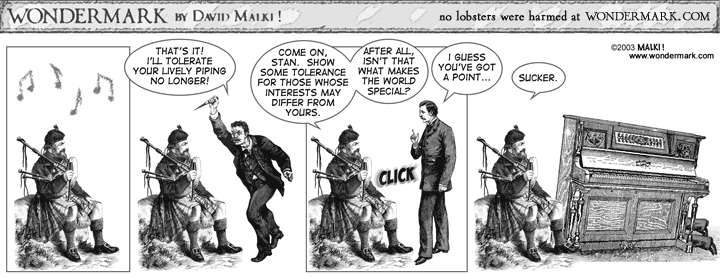
\includegraphics[width=0.9\textwidth]{bilder/comics/wondermark003.png}
\end{figure*}

% TODO sind die Begriffe, die man für den Studienplan braucht, hier gut untergebracht oder sollten die mit in den restlichen Erklärungstext? Ist das hier wirklich eine kurze, neutrale Begriffserklärung oder nicht eher ein Kapitel "Kritische Kommentrare zu den Vorlesungen und Übungen"?

Einen guten "Uberblick "uber die an der Uni gebr"auchlichen Begriffe und
Abk"urzungen findest du im "`Uni-ABC"' des AStA-Erstiinfos. Im folgenden
sind nur die wichtigen Begriffe f"ur deinen Stundenplan erkl"art, den du
auf der letzten Seite dieses Heftes findest.




% TODO Spätestens hier (Noch Fragen?) hört's auf, die Fragen sind keine Begriffsklärung mehr. Das ist ja gut, dass es solche Texte gibt, aber die Überschrift passt einfach nicht.
\subsubsection*{Noch Fragen?}

Die Qualit"at dieser drei Veranstaltungsarten ist in starkem Ma"se vom
jeweiligen Vortragenden abh"angig. W"ahrend du unter Umst"anden die
Seminargruppen noch wechseln kannst, so ist das bei den erstgenannten
Veranstaltungen nat"urlich nicht m"oglich.

Du wirst sehr bald feststellen, dass es verschiedene Lerntypen gibt. Manche
deiner Kommilitonen werden kaum eine Vorlesung besuchen, sondern stattdessen die gro"sen
und kleinen "Ubungen verschlingen. Wieder andere lassen sich sowieso kaum im
H"orsaal blicken, sondern k"onnen am besten zu Hause oder in der Uni-Bibliothek
autodidaktisch lernen.

Wenn trotz Vorlesungen, gro"ser "Ubungen und kleiner "Ubungen noch Fragen
auftreten, so hilft dir das Gespr"ach mit den Kommilitonen oder der Blick in
entsprechende Literatur.
Wichtig: Kaufe nicht gleich jedes empfohlene Buch neu,
das ist Geldverschwendung. Frage h"ohere Semester nach wirklich sinnvoller
Literatur, leih' dir die B"ucher aus der UB aus, gebrauchte B"ucher gibt es
g"unstig z.B. in der Newsgroup \nurl{http://groups.google.de/group/braunschweig.kaufrausch/} (siehe den Artikel
ab Seite \pageref{elekinf}). An der Uni wird man nicht umsorgt wie etwa in der
Schule oder in der betrieblichen Ausbildung, du tr"agst ein wesentlich h"oheres
Ma"s an Eigenverantwortung. Zur Orientierung in der ersten Zeit ist ein
Ansprechpartner unentbehrlich. Wenn die Kommilitonen aus
deinem eigenen Semester nicht weiterhelfen k"onnen, dann vielleicht dein/e TutorIn oder andere
Studierende im h"oheren Semester (zum Beispiel Mitbewohner, Fachgruppe).
